\chapter{Results and analysis}

\section{Classification impovements}

Did classification improve, how, why

\begin{figure}[ht!]
  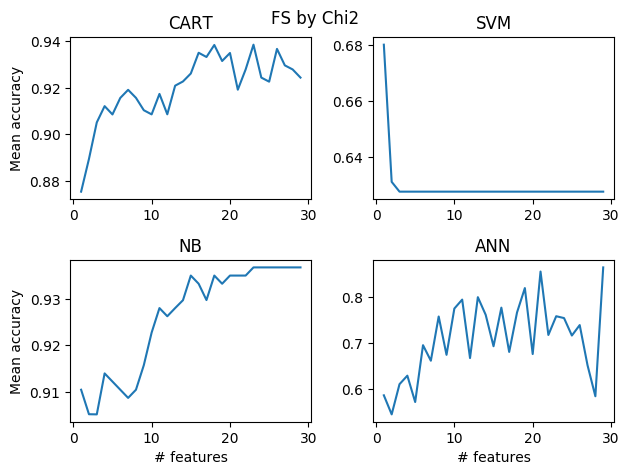
\includegraphics[width=\linewidth]{../plots/FS_by_Chi2.png}
  \caption{Performance by selecting features by Chi2}
  \label{fig:chi2}
\end{figure}

\begin{figure}[ht!]
  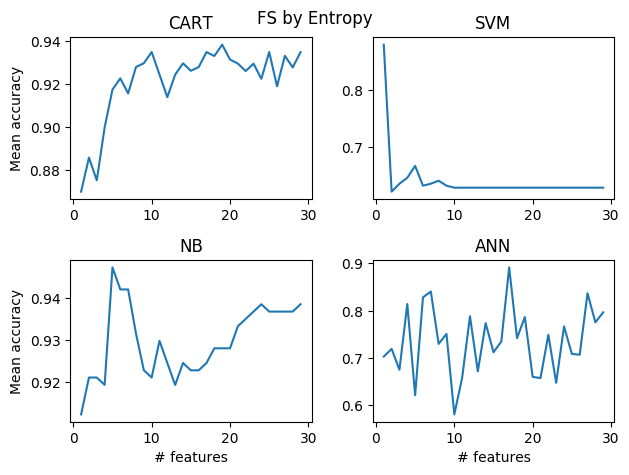
\includegraphics[width=\linewidth]{../plots/FS_by_Entropy.png}
  \caption{Performance by selecting features by Entropy}
  \label{fig:entropy}
\end{figure}

\begin{figure}[ht!]
  
\includegraphics[width=\linewidth]{../plots/RFS.png}
  \caption{Performance by selecting features by RFS}
  \label{fig:rfs}
\end{figure}

\section{Best features}

Could we tell which features contributes most to correct classification, how, why those

\section{Source of errors}

What can have caused faulty results, can our results be trusted?
